\documentclass[a4paper,10pt]{report}

% Language
\usepackage[UKenglish]{babel}    % define culture for rendering (eg., hyphenation rules)
\usepackage[T1]{fontenc}       % use utf8 fonts
\usepackage[utf8]{inputenc}      % input encoding is utf8
\usepackage{lmodern}             % use font Latin Modern

% Supreme boilerplating
\usepackage{etex}                % LaTeX 2.0 features on relics
\usepackage{microtype}           % Extremely anal typographic mode
\usepackage{url}                 % Ability to create URLs
\usepackage[hidelinks]{hyperref} % Makes intradocument links, eg., contents page
\usepackage{color}               % Adds colour features. Really.
\usepackage{graphicx}            % Adds image features

% Layout
\usepackage[a4paper]{geometry}   % In case I want to set margins etc.
\usepackage{setspace}            % For setting line spacing
\usepackage{enumerate}           % Allows different types of numbering
\onehalfspacing

% Actual Packages
\usepackage{fixme}
\usepackage[authoryear, round, sort]{natbib} % References
\usepackage{amsmath}             % Imports for maths things
\usepackage{amssymb}
\usepackage{amsthm}
\usepackage{empheq}              % For highlighting mathematics
\usepackage{tikz}
\usetikzlibrary{arrows,shapes,decorations.pathreplacing,decorations.pathmorphing,calc,patterns,scopes,trees,positioning,fit}
\usepackage{pgfplots}
\pgfplotsset{compat=1.7}
\pgfkeys{/pgf/number format/relative round mode=fixed}

% Bug Fixes
\usepackage{fixltx2e}            % LaTeX bugfixes (yes really)
% "fix the natbib spacing character" - Kevin Naud�
\makeatletter
\ifdefined \NAT@spacechar
	\def\NAT@spacechar{~}
\fi
\makeatother

\hypersetup{pageanchor=false}    % Wait until actual start of writing before making page anchors


%%%%%%%%%%%%%%%%%%%%%%%%%%%%%%%%%%%%%%%%%%%%%%%%%%%%%555
% Macros

% Restarts numbering and sets format to 1, 2, 3...
\newcommand \startrealnumbers { 
	\pagenumbering{arabic}
	\setcounter{page}{1} 
	\hypersetup{pageanchor=true}
}

% Renders a bibliography on its own page, and adds a contents reference.
\def \bibliographysection {
	\cleardoublepage
	\phantomsection
	\addcontentsline{toc}{chapter}{Bibliography}
	\bibliographystyle{authordate3}
	\bibliography{bibliography}
}

\newcommand \todo \fxwarning

\begin{document}

\title{A JIT-less, Register-Mapped, Statically-Typed Virtual Machine for Interpreters}
\author{Matthew Sainsbury}
\date{\today}

% Cover Page
\begin{titlepage}

		\maketitle
	
\end{titlepage}

\pagenumbering{roman}

% Prefaces
\nakedchapter{Acknowledgements}
	I acknowledge Douglas Bentley for his help drafting the virtual machine's architecture, writing benchmarks for their evaluation, and staying sane. Douglas is researching other interesting ideas in virtual machine design, and we collaborated to produce a shared set of benchmark programs for our virtual machines.
	
	I acknowledge Kevin Naudé for his role as my honours supervisor.
	
	The practical components of this project made extensive use of GNU software provided by the Free Software Foundation.
	
	The financial assistance of the National Research Foundation (NRF) towards this research is hereby acknowledged. Opinions expressed and conclusions arrived at, are those of the author and are not necessarily to be attributed to the NRF.

\nakedchapter{Abstract}
	Conventional JIT-less high-level register virtual machines simulate virtual registers in random access memory (RAM) and load virtual registers from RAM whenever they are accessed \citep{caseregistervm}. This treatise investigates an alternative approach where virtual registers are mapped to physical registers, and instructions are dispatched not only on the opcode, but also on the register operands of the instruction. To emulate a virtual instruction, the interpreter jumps to the appropriate code segment in a table of implementation code based on the instruction word to be executed. This table is very large, and therefore the performance implications of this approach is investigated.

\nakedchapter{Declaration of Own Work}
	I declare that the entirety of the work contained in this treatise is my own, original work, that I am the sole author thereof (save to the extent explicitly otherwise stated), that reproduction	and publication thereof by Nelson Mandela Metropolitan University will not infringe any third	party rights that I have not previously in its entirety or in part submitted it for obtaining any qualification.
	
	\vskip 1em
	
	Signature: \underline{\hspace{3cm}}
	
	Date: \today

\singlespacing
\tableofcontents
\onehalfspacing

% Main document body
\chapter{Introduction}
	\startrealnumbers
	Interpreters are a popular way to implement programming languages. They allow programs to be portable, and, compared to natively compiled programs, more readily support advanced features like debuggers. 
	
	Virtual machines are commonly used in the implementation of interpreters. Virtual machines provide an abstraction layer between the interpreted program and the host machine. This abstraction hides each specific host machine's details, and affords interpreted languages their portability. The abstraction also eases implementation by providing a ``stepping stone'' between the high-level ideas of a programming language and the low-level details of the processor.
	
	Compared to native execution, interpretation does add significant overhead to the execution of programs. Research effort has been expended to optimise virtual machines for interpreters, but much of this research was done on older processors which no longer reflect the structure of modern designs. For instance, modern processors have far larger cache sizes than the processors of previous generations.
	
	This treatise investigates a new implementation technique for virtual machine interpreters that run on modern processors. Two ideas are presented: register mapping between virtual machine registers and real registers, and a new dispatch method which operates on full instruction words. 
	
	The goal of this research is to determine whether these two ideas can contribute to a new virtual machine design that is better designed for modern processors than conventional VMs. This chapter aims to establish the landscape of modern processor design and the problems which arise in virtual machine implementations, as well as describe the scope of this project.
	
	\section{Background}
		A virtual machine is a program that executes other programs by emulating the instruction-level behaviour of a chosen machine. In some cases, virtual machines allow programmers to execute programs written for one kind of computer on a machine that has an unrelated architecture. In other cases, virtual machines run programs designed for theoretical machines for which no physical devices exist to execute them.
		
		Virtual machines designed to emulate theoretical machine are known as high-level virtual machines. These kinds of virtual machine may sound worthless to someone who has only been exposed to the more immediately visible applications of virtual machines, like playing games designed for obsolete game consoles, but high-level virtual machines serve as convenient and powerful design patterns in high-level programming language interpreters.
		
		A high-level virtual machine runs programs for a machine which is imagined by its designer. Because it is not bound by the practical limitations of machines with real implementations, it may have more sophisticated features and other desirable properties which would be difficult to build into a real machine. An high-level virtual machine can be considered to be an abstraction layer that hides the intricacies of any particular real machine. A further advantage is that virtual machines can be implemented on any physical architecture, resulting in the extremely useful property that code written for a virtual machine is very portable. The portable ``machine code'' that high-level virtual machines execute is usually called its \emph{bytecode}. 
		
		The primary use for high-level virtual machines is in high-level interpreted languages, such as Java and Python. High-level language interpreters are typically implemented with a compiler that compiles the input source code into an intermediary bytecode, which is then interpreted on a high-level virtual machine. This kind of interpreter executes programs much faster than interpreting the source code line-by-line.
		
		Virtual machines also offer software engineering benefits for implementing interpreters. Writing a compiler flexible enough to target many machines with vastly different designs is difficult, and especially difficult for modern, complex high level languages. A high-level virtual machine allows a compiler that targets a single, albeit virtual, platform while still retaining the portability of the system. It is easier to re-target a virtual machine for a new architecture than an entire compiler. Ease of compiler implementation is increased by the high-level nature of the virtual machine, which can support instructions for complex tasks that would be difficult to compile down to native machine code. From an architectural design point of view, virtual machines help keep interpreters internally organised. Interpreter developers can seperate the language and context analysis functions---which remain in the compiler---from the host-specific implementation details which are compartmentalised into the virtual machine \citep{structureinterpreters}.
		
		Interpreters implemented with virtual machines are among the fastest kinds of interpreters \citep{modernarchvm}. However, they remain significantly slower than executing native code \citep{optimizingindirectbranch}. An important and widely used optimisation technique for virtual machine interpreters is Just-in-time (JIT) compilation. JIT is not explored in this research, but is a relevant and complementary technique. JIT tries to bring ``the best of both worlds'' together. Modern JIT interpreters execute an instrumented interpreter which gathers profiling data to determine which parts of the bytecode would most benefit from native execution. Once it has identified these sections of bytecode, it compiles them into the host machine's instruction set and executes them natively instead of interpreting them \citep{historyjit}. Most popular virtual machines utilise JIT compilation, such as Java's JVM.
		
		JIT compilation is a good strategy to improve the performance of virtual machines, but it has disadvantages in certain use cases. An example is found in multi-instance programs, where a program is started many times, concurrently, so that multiple instances run as separate processes at the same time. In such cases, JIT compilation results in repeated work, and reduced memory sharing. A practical example of such a program is in a PHP web server, which spawns several identical program instances to serve web clients asynchronously.
		
		Operating systems allow distinct processes to share memory under certain conditions. If two processes load the same resource into read-only memory blocks, the resource can be loaded into one memory location which is shared by both processes. This mechanism is automatic and transparent to the process as long as the memory blocks concerned are read-only and cannot be altered by the other process. An example of this in action is shown in \reffig{nativeprogram}, where two instances of the same program share a read-only code space in memory \citep{sharedcodepatent}. 
		
		The sharing of memory in the context of JIT-enabled interpreters is complex. When two instances of a JIT interpreter are started, they both load the interpreted program into memory. However, since JIT is a rewriting process, the two processes cannot share JIT data, because the operating system cannot negotiate transparent sharing of writeable memory blocks. Each interpreted process utilising JIT must do its own tracing and JIT compilation of the bytecode. In multi-instance programs, this results in the same code being compiled over and over again (\reffig{interpretedprogram}) and the produced code is not shared. JIT compilation is a hefty procedure, so multiple compilations of identical code is undesirable. 
		
		\begin{doublefig}
			\begin{halffig}
				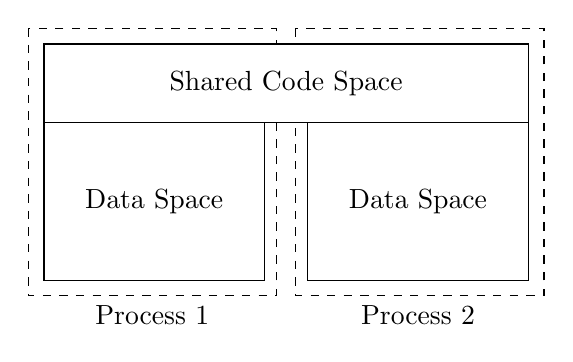
\begin{tikzpicture}
				\draw (-0.2, 0.2) [dashed] rectangle (2.95, -3.2) node[below] at (1.375, -3.2) {Process 1};
				\draw (3.2, 0.2) [dashed] rectangle (6.35, -3.2) node[below] at (4.75, -3.2) {Process 2};
				\draw (0,0) [fill=white] rectangle (6.15,-1) node[midway] {Shared Code Space};
				\draw (0,-1) rectangle (2.8, -3) node[midway] {Data Space}; 
				\draw (3.35,-1) rectangle (6.15, -3) node[midway] {Data Space}; 
				\end{tikzpicture}
				\caption{Two native programs}
				\label{fig:nativeprogram}
			\end{halffig}
			\begin{halffig}
				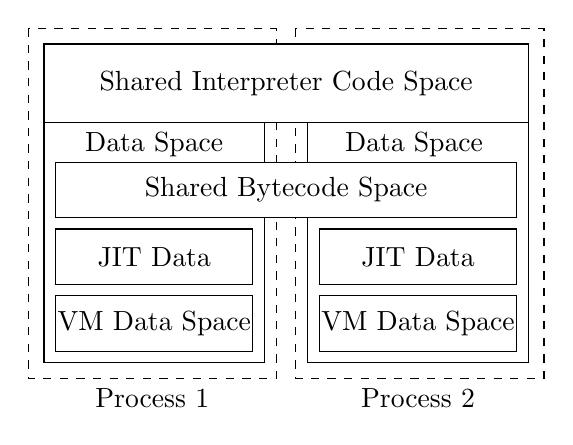
\begin{tikzpicture}
				\draw (-0.2, 0.2) [dashed] rectangle (2.95, -4.25) node[below] at (1.375, -4.25) {Process 1};
				\draw (3.2, 0.2) [dashed] rectangle (6.35, -4.25) node[below] at (4.75, -4.25) {Process 2};
				\draw (0,0) [fill=white] rectangle (6.15,-1) node[midway] {Shared Interpreter Code Space};
				\draw (0,-1) rectangle (2.8, -4.05) node[below] at (1.4,-1) {Data Space}; 
				\draw (3.35, -1) rectangle (6.15, -4.05) node[below] at (4.7,-1) {Data Space};
				\draw (0.15, -1.5) [fill=white] rectangle (6, -2.2) node[midway] {Shared Bytecode Space};
				\draw (0.15, -2.35) rectangle (2.65, -3.05) node[midway] {JIT Data};
				\draw (3.5, -2.35) rectangle (6, -3.05) node[midway] {JIT Data};
				\draw (0.15, -3.2) rectangle (2.65, -3.9) node[midway] {VM Data Space};
				\draw (3.5, -3.2) rectangle (6, -3.9) node[midway] {VM Data Space};
				\end{tikzpicture}
				\caption{Two interpreted programs}
				\label{fig:interpretedprogram}
			\end{halffig}
		\end{doublefig}
		
		Multi-instance applications have become more common, as CPUs increase in core count. Since the popular approach of JIT compilation is unsatisfactory in this use case, it is worthwhile to explore efficient virtual machine designs which do not require JIT compilation, which is the subject of the present research. This research falls into this area of interest. To facilitate dialogue in the space of non-JIT virtual machines, an exposition of conventional virtual machine implementation techniques for modern architectures is now presented.
		
		\subsection{Conventional Virtual Machines}
			There are two common types of high-level virtual machine architectures: stack machines and register machines. Stack machines store temporary values in a stack data structure, while register machines store temporary values in storage ``boxes'' called registers. Both machine classes utilise a call stack to provide function call handling and return. In a stack machine, the call stack and temporary variable store are unified. In a register machine, the call stack is a secondary  structure.
			
			\subsubsection{Stack Machines}
			Most of a stack machine's instruction set consists of operations on the stack. \reffig{stackprogram} shows an example of code written for a stack machine. Notice that the operands of the instructions (such as \texttt{add} and \texttt{divide}) are implicit, and so instructions for stack machines tend to be shorter. The complexity of individual instructions is a major difference between stack machines and register machines. 
			
			Each instruction in a program is encoded as a series of bytes called an \emph{instruction word}. The component of the instruction word which specifies the operation to be performed (eg., \texttt{add}) is called the \emph{opcode}. 
			
			In a stack machine, the instruction encoding is simple. Each opcode is assigned a unique instruction code. For instance, the program listed in \reffig{stackprogram} might be represented as in \reffig{stackencoding}. Notice how constant operands are appended to the end of the instruction. This extra data is known as an immediate.
			
			\begin{doublefig}
				\begin{halffig}
					\begin{lstlisting}
push 14
push 8
add
push 7
div
print
					\end{lstlisting}
					\caption{Stack machine program to calculate $(14+8)\div7$}
					\label{fig:stackprogram}
				\end{halffig}
				\begin{halffig}
					
					\texttt{
						\begin{tabular} {| l | l |}
							\hline
							Encoding & Instruction \\
							\hline
							0x01 0x0E & push 14\\
							0x01 0x08 & push 8\\
							0x00 & add \\
							0x01 0x07 & push 7\\
							0x02 & div \\
							0x03 & print \\
							\hline
						\end{tabular}
					}
					\caption{Stack Instruction Encoding}
					\label{fig:stackencoding}
				\end{halffig}
			\end{doublefig}
			
			\subsubsection{Register Machines}
			The instructions of a register machine stand in contrast to that of a stack architecture in that the operands are always explicitly specified. \reffig{registerprogram} shows the same program for a register machine. Here, the \texttt{add} instruction is annotated to specify that the value of \texttt{regA} is added to \texttt{regB}, and the result is stored in \texttt{regA}.
			
			\begin{doublefig}
				\begin{halffig}
					\begin{lstlisting}
mov regA, 14
mov regB, 8
add regA, regB
mov regB, 7
div regA, regB
print regA
					\end{lstlisting}
					\caption{Register machine program to calculate $(14+8)\div7$}
					\label{fig:registerprogram}
				\end{halffig}
				\begin{halffig}
					\texttt{
						\begin{tabular}{ | l | r | r |r |}
							\hline
							Meaning & opcode & dest & src  \\ 
							\hline
							movc regA & 0000 & 0000 & 0000  \\
							\hline
							(extra: 14) & 1110 \\
							\hline
							movc regB & 0000 & 0001 & 0000  \\
							\hline
							(extra: 8) & 1000 \\
							\hline
							add regA, regB & 0001 & 0000 & 0001   \\
							\hline
							movc regB & 0000 & 0001 & 0000  \\
							\hline
							(extra: 7) & 0111 \\
							\hline
							div regA, regB & 0002 & 0000 & 0001  \\
							\hline
							print regA & 0003 & 0000 & 0000  \\
							\hline
						\end{tabular}
					}
					\caption{Register Instructions as Bitfields}
					\label{fig:bitfields}
				\end{halffig}
			\end{doublefig}
			
			A register machine's instruction encoding is more complicated because the operands of the instruction need to be part of the instruction encoding. The conventional implementation uses bitfields. The first few bits are reserved for encoding the opcode, which follows the same format as with a stack machine. The rest of the bits are divided into segments, into which each register operand is encoded. For example, consider a twelve-bit instruction word. The first four bits can be reserved for the opcode, allowing for up to 16 unique opcodes. The next four bits of the instruction word can encode the first operand register number as an enumeration, and the last four bits can encode the second operand register number. If an instruction only has one operand, the last four bits are undefined. Immediate values may either form part of the instruction word, or follow it as a disitinct value. An encoding solution for \reffig{registerprogram} appears in \reffig{bitfields}. Notice how `\texttt{mov regA, 14}' has been transformed into `\texttt{movc regA}' followed by an immediate value. Whether an instruction is interpreted as having an immediate value depends on the interpretation of the instruction, so it is necessary for the instruction implementation to expect to find an immediate adjacent to it, otherwise the immediate would be treated as an instruction. This is why the \texttt{movc} (move constant) instruction was invented for this example.
			
			Real register machines implement registers in high-speed memory hardware as part of their design. However, virtual machines have difficulty emulating high-speed registers because virtual machine registers are typically stored in the host's (slower) main memory.
			
			
		\subsection{Modern Processors}
			The landscape of processor design has changed significantly in the last thirty years. Rather than producing performance gains by increasing processor clock speeds, modern processor designers rely on increasing the instruction-per-cycle efficiency of their processors. The enabling techniques include instruction pipelining, larger and more complex cache systems, multiple issue and speculative execution. These new design ideas caught the interest of academics and engineers in the 1980's \citep{modernprocessordesign}. Some of these new processor features significantly alter the performance characteristics of virtual machine interpreters, and are briefly discussed in this section.
			
			\subsubsection{Cache Arrangement}
			Modern processors contain portions of high-speed memory which act as a cache to the main memory of the machine. The behaviour of this cache is an important factor for processor performance, because main memory is quite slow compared to the speed of a CPU. Modern caches are orders of magnitude larger than those available in processors twenty years ago. 
			
			Most modern processors contain a series of specialised caches. For instance, a fourth-generation Intel Core processor has at least three grades or \emph{levels} of cache, and make a distinction between cache for instructions and cache for program data. \reffig{cachenumbers} shows the arrangement of cache on such a processor. As can be seen, L1 cache is much faster, but much smaller than L2 cache. The latency in L1 instruction cache is not reported because instruction fetch is transparent to programs, but it does influence the speed of execution through the process of instruction pipelining (see~later). It is advantageous for a program if most of its application data can fit in L1 data cache, and most of its active code can fit in L1 instruction cache. However, conventional virtual machines have not been designed to take advantage of the large amount of cache available on modern processors.
			
			\begin{myfigure}
				\begin{tabular}{ | l | l | l | l | }
					\hline
					Level & Type & Size & Latency \\ 
					\hline
					\multirow{2}{*}{L1} & Instruction & 32KB & N/A \\
					& Data & 32KB & 4 cycles \\
					\hline
					L2 & Data & 256KB & 11 cycles \\
					\hline
					L3 & Data & Varies & Varies \\
					\hline
				\end{tabular}
				\caption{Cache on 4th-Gen Intel Core CPUs \citep{optimisationreference}}
				\label{fig:cachenumbers}
			\end{myfigure}
			
			\subsubsection{Instruction Pipelining}
			Early processors executed machine instructions one at a time. Each instruction would occupy the CPU for some number of cycles, as it was fetched, decoded and executed. The result of this method is that each instruction would move through a sequence of activity stages, but only one stage of the process would be ``working'' at any time. For instance, when an instruction was being decoded, the entire execution component of the processor was unused.
			
			On a processor with pipelining, these independent operations are overlapped in time. An instruction can be fetched while another instruction is being decoded, and yet another instruction's operands are being fetched. A processor that can operate this way is said to have an \emph{instruction pipeline.} This results in far better utilisation of processor hardware. It also introduces complexity in the processor design. For instance, if one instruction writes to a memory address, and later instruction reads from the same address, the second instruction cannot complete the operand fetch stage until the first instruction has been executed. A situation where an instruction has to wait for another to complete is known as a \emph{pipeline stall,} and is a subject of much academic writing and engineering effort. Modern processors try to avoid stalls by predicting in advance what data is likely to be needed, or forwarding results backwards in the pipeline to fetch stages. Pipelining is an important consideration in the design of virtual machines, especially with predicting the behaviour of branches.
			
			\subsubsection{Branch Prediction \& Branch Target Prediction}
			Branch prediction in a process refers to the processor's ability to continue the pipelining process during a branch instruction. Ordinarily, the location of the next instruction is known to the processor---it is simply the instruction adjacent to the previous one. If the previous instruction was an instruction to branch (go somewhere else in the program), the picture becomes more~complex. There are three types of branches worth mentioning:
			\par\nobreak\makeatletter\@afterheading\makeatother
			\begin{description}
				\item[Unconditional Branch:] This instruction always causes the processor to jump to the same location. The target of the branch is known as soon as the instruction is decoded.
				\item[Conditional Branch:] This branch type branches to one of two locations, depending upon a breaking condition---for instance if a register is zero (``branch if zero''). The location of the next instruction is only known once the branch instruction has evaluated the condition, but some processors try to predict which location will be selected.
				\item[Indirect Branch:] A branch whose target location is based on program data, whether in memory or in a register, or both. The branch is always taken, but the destination is not known in advance. Indirect branches are very difficult to predict because they are determined by arbitrary data.
			\end{description}
			
			An unconditional branch is the easiest branch to pipeline, since the location of the next instruction is encoded in the branch instruction itself, and the target location does not change. The next instruction can be fetched as soon as the branch instruction is decoded. 
			
			A conditional branch is harder to pipeline because it is not known whether the condition is true or false before the instruction is executed, and hence the branch target is discovered too late. To prevent pipeline stalls on conditional branch instructions, modern processors implement a \emph{branch predictor}. The branch predictor will use some heuristic to predict the conditional, and load the most likely next instruction. A pipeline stall will only occur if the prediction is wrong---this delay is known as the \emph{misprediction penalty}.
			
			An indirect branch is the worst type of branch for a pipelined processor. It is very hard to predict because the branch location could depend on any data anywhere in main memory or in registers. This influence that data has on the behaviour of the program is known as \emph{data dependance} and is to be avoided whenever possible. Modern processors implement a \emph{branch target predictor} in an attempt to reduce the number of pipeline stalls for indirect branches. A branch target predictor is not to be confused with a branch predictor---a branch predictor predicts whether the branch will be taken, whereas a branch target predictor tries to predict where the branch will lead. A conditional branch can only lead to one of two places---the next instruction, or the constant branch location; whereas an indirect branch could lead anywhere.
			
			One common branch target predictor is a \emph{branch target buffer} (BTB). A branch target buffer maintains a table storing the last target location of each indirect branch encountered. A BTB makes the assumption that an indirect branch target is unlikely to change  \citep{yeti}, and uses the table to make a prediction of where a specific indirect branch will go. This strategy works well if an indirect branch always branches to the same location, but is no help if it is always different.
			
			Indirect branches are a big issue in virtual machine design, since an indirect branch is unavoidable during the dispatch process of a virtual machine \citep{structureinterpreters}. Nevertheless, it may be possible to significantly increase the dispatch performance of a virtual machine by increasing the likelihood that indirect branches are predicted correctly by a branch target predictor. These concepts form the background to this research, and the problems which motivate it.
	
	\section{Problem Description}
		Most physical computational machines are register machines. It is thought that the use of real machine registers to store the values of the virtual machine registers will help to make the operation of virtual machine programs more transparent to the physical CPU by reducing data-dependant fetches from main memory, where virtual machine registers are usually stored. Unfortunately, unlike virtual registers that are implemented in memory, real registers cannot be accessed by dynamic index \citep{caseregistervm}. This difference complicates the implementation of a register-mapped virtual machine. Nevertheless, there may exist techniques to exploit modern processor features to obtain register-mapping. It is worthwhile to investigate designs of JIT-less register virtual machines that attempt to narrow the divide between the host and guest architecture.
		
	\section{Purpose and Scope}
		The goal of this project is to investigate the feasibility of JIT-less register virtual machines for interpreters running on a modern architecture. To this end, a high-level register virtual machine will be implemented with some unique architecture features that have not been investigated or thought feasible previously. The virtual machine will be developed for a statically typed language. Consequently, the virtual machine does not have to perform type checking on operands.
		
		A novel dispatch process will be investigated that seeks to allow the use of physical machine registers in the implementation of virtual machine registers. To circumvent the problem of referencing real machine registers, the virtual machine will dispatch not only based on the opcode of each instruction, but on the instruction as a whole. In other words, an implementation will exist for every combination of operands in each virtual machine instruction.
	
		An instruction set architecture will be designed which will be tailored for such a dispatch method. It is anticipated that having implementations for every combination of operands in each virtual machine instruction will cause the virtual machine implementation to become very large, and so the design of the instruction set architecture will focus on keeping the number of unique instructions low. The number of registers exposed by the VM architecture may have to be restricted to reduce the number of operand combinations in instructions.
		
		The relationship between the number of registers, number of distinct operations, and the size of the VM code can be shown mathematically. Assuming any virtual machine register can be used as an operand for any instruction, the size of the virtual machine implementation is proportional to:
		
		\[
		\sum_{p~\in~opcodes} r^{n(p)} : 
		\begin{array}{l}
		n(p) \coloneqq \text{number of operands for $p$} \\
		r \coloneqq \text{number of virtual machine registers}
		\end{array}
		\] 
		
		Consequently, every additional virtual machine register increases the size of the virtual machine by a polynomial factor. At some point, any performance gain received by exposing more physical registers will be negated by increasing incidence of cache misses. For this reason, the number of exposed registers must be limited. The extent to which such constraints are of practical value to the virtual machine performance must be determined.
		
		As the virtual machine implementation becomes very large, it may become unsuitable for operation on machines with small L1 and L2 instruction caches. This is the case if the cache is inadequate to host large portions of the active virtual machine implementation. If this is to occur, the virtual machine may actually be slower than conventional virtual machines. Hence, the design will consider only modern processors with reasonably large first-level cache, such as the fourth-generation Intel Core i7 range of processors which contain 32KB of L1 instruction cache.
				
	\section{Overview of Treatise Structure}
		This treatise documents the process of evaluating new ideas in virtual machine design. In Chapter~2, an outline of relevant research in the field of virtual machine and interpreter design is presented. A small amount of related work has previously been done, which will be highlighted. This chapter forms a framework around which the new design is presented in Chapter~3.
		
		Chapter~4 describes how those ideas are evaluated in a series of empirical tests and benchmarks. The results of these benchmarks are presented and discussed. Final conclusions and discussion are found in Chapter~5, along with recommendations for future work.

% 10-12 pages
\chapter{Problem Exposition}
	\section{Literature Review}
		\cite{structureinterpreters} reflect on why spending research and engineering effort on optimising interpreters is a worthwhile endeavour. Creating a machine abstraction layer between original source code and host machine architecture greatly simplifies the writing of compilers that target many platforms. Without such an abstraction layer for each host machine, a separate version of the compiler targeting that platform must be developed. Interpreters allow compilers to be more versatile with little effort. In a high-level language interpreter utilising a virtual machine, only the interpreter portion needs to be rewritten for different platforms, (or perhaps not even the interpreter if a high-level language is used to implement the interpreter) and the compiler remains the same. Interpreters tend to be simple compared to compilers targeting machine code, so this advantage is quite significant. Compared to native execution, interpreters also offer opportunity for more powerful usability features like debuggers, and have faster compilers, improving the write-compile-test cycle of modern software development methods.
		
		The benefits of using interpretation comes at some cost in performance. A program running on virtual machine is about 5--10 times slower than the same program running natively~\citep{optimizingindirectbranch}. This cost may be much larger if the design of the interpreter is poor. A well-designed high-level virtual machine is both easy to compile code for (sophisticated) and allows for fast interpretation (low overhead). Such consideration should be applied aross all features of an interpreter.
		
		\cite{fastjava} believes that interpreters are not well designed to suit modern architectures features like pipelining, branch prediction and caches. They also provide encouragement by saying, ``if interpreters can be made much faster, they will become suitable for a wide range of applications that currently need a JIT.'' \cite[]{structureinterpreters} says that the performance difference between inefficient and efficient interpreters is larger than the difference between efficient interpreters and native code.
		
		\subsection{Virtual Machine Dispatch}
		One feature that is present in all virtual machine interpreters is an instruction dispatch process. Dispatch refers to the process of fetching, decoding, and starting the execution of the code that is specific to the next virtual machine instruction. The dispatch technique can have the biggest effect on the performance of a virtual machine because it operates for every VM instruction executed. Consequently, interpreters spend most of their execution time on instruction dispatch \citep{modernarchvm}. 
		
		There are a variety of widely known implementation techniques for instruction dispatch. The fastest know dispatch method is direct threaded code~\citep{structureinterpreters}. ``Threading'' in this case does not refer to ``multithreading'', but instead to a much older type of code structuring technique. In this method, a virtual machine instruction is actually the address of the code that implements that instruction. This is illustrated in \reffig{directthreading}. Notice the line `\texttt{jmp *pc++}'. This is an indirect branch. An indirect branch is an inescapable consequence of the dispatch process. Direct threading is efficient because, although it contains an indirect branch, there is little other overhead. Techniques for improving the accuracy of branch target prediction have been investigated, and some more interesting ones are summarized by \cite{optimizingindirectbranch}. 
		
		\begin{myfigure}
				\begin{lstlisting}
start:
  pc = bytecode
  jmp *pc++

bytecode:
  &add
  &divide
  &print

add:
  //implementation
  jmp *pc++

divide:
  //implementation
  jmp *pc++

print:
  //implementation
  jmp *pc++

				\end{lstlisting}
				\caption{Direct Threading Dispatch}
				\label{fig:directthreading}
		\end{myfigure}
		
		Note that the jump instruction is duplicated at the end of each instruction. The reason is that duplicating the indirect branch increases the utilisation of a branch target prediction, since there is an entry in the branch target buffer for each source address of an indirect branch. If instead one common jump instruction is used, the BTB would always predict that the next instruction is the same as the previous one, which is almost always incorrect. This will be better explained later in this chapter.
		
		An interesting finding of \cite{optimizingindirectbranch} is that branch prediction in loops can be greatly improved if every instruction within the loop body is unique. Branch prediction accuracy can be perfect in that case, because the current instruction is always sufficient to predict the next instruction. 
		
		Consider the code in \reffig{duplicatedinstructions}. During the second iteration of the loop, after the A instruction, C will be predicted because it was the last instruction to follow A. This is incorrect because B is the next instruction. The BTB will be updated to reflect that B follows A. After the next A instruction, B will be predicted because it was the last instruction to follow A. However, this is wrong again, and the BTB will update its prediction once more. A misprediction happens after every A instruction.
		
		However, if the A instruction implementation is duplicated to produce A1 and A2, as in \reffig{deduplicatedinstructions}, a different pattern emerges. During the second iteration of the loop, after the A1 instruction, B will be predicted. C is no longer predicted because this instruction only follows A2. This loop is perfectly predicted after the first iteration. An implementation of this technique is discussed in the next section
		
		\begin{doublefig}
			\begin{halffig}
				\begin{lstlisting}
loop:
  A
  B
  A
  C
jmp loop
  				\end{lstlisting}
				\caption{Loop With a Duplicated Instruction}
				\label{fig:duplicatedinstructions}
			\end{halffig}
			\begin{halffig}
				\begin{lstlisting}
loop:
  A1
  B
  A2
  C
jmp loop
				\end{lstlisting}
				\caption{Loop with De-duplicated Instructions}
				\label{fig:deduplicatedinstructions}
			\end{halffig}
		\end{doublefig}
		
		
		
		Another interesting technique investigated by \citeauthor{optimizingindirectbranch} is the use of `superinstructions' which are groups of instructions with a single opcode. Combining instructions into more complex instructions can reduce branch prediction failures by increasing the variety in opcodes. It also reduces the number of indirect branches, because a dispatch no longer occurs between the instructions that have been combined into a composite instruction. For instance, superinstructions can be applied to \reffig{duplicatedinstructions} by combining the (A, C) instruction pair into an instruction AC. This results in a perfect prediction in this instance.
		
		Traditionally, the high level virtual machines implemented in interpreters are stack machines. Stack machines have been favoured over register machines for a few reasons. Instructions for stack machines are smaller, because instruction operands are implicit. This means that instruction fetching is faster. It is easier to compile code for a stack machine than a register machine because the compiler does not need to implement a register allocator \citep{caseregistervm}. However, \cite{stackregistershowdown} found that an efficient register virtual machine can execute benchmarks 32\% faster than an analogous stack machine. 
		
		There might be historic factors involved in the prevalence of stack based virtual machines. \cite{caseregistervm} mentions that the first successful virtual machine interpreter ran stack-based P-code for Pascal. This was the first in a large family of stack-based bytecodes for popular languages like Smalltalk, Java and the Common Intermediate Language (CIL).
		
		\subsection{Relevant Previous Work}
		\cite{optimizingindirectbranch} discuss a technique they call dynamic replication, which solves the problem described in the previous section where duplicate instructions in a loop result in large amounts of misprediction. In this technique, the interpreter dynamically adds duplicates of instruction implementations to the virtual machine for each instruction emitted by the compiler. The bytecode produced by an interpreter utilising this technique consists of no duplicate opcodes, because if two of the same instruction exist, they will correspond to different implementation instances in the virtual machine. This technique dramatically reduces indirect branch mispredictions at the cost of increased code size.
		
		The practice of mapping virtual machine resources to host machine registers has been investigated for stack machines by \cite{stackcaching}. Ertl measured the performance of stack machines which kept the top few elements of the stack in registers. For the case of static register assignment, Ertl found that direct mapping of stack positions to machine registers was only useful for the case where just the top element of the stack was cached in a register. Further caching resulted in too many load-store instructions to shuffle register values around when positions on the stack change.
		
		Ertl also attempted a technique he calls ``dynamic stack caching'' where stack elements are cached in whatever register is convenient, and an internal state machine remembers the mapping between stack context and registers. The technique employs multiple versions of code to emulate each virtual machine instruction; the version which is executed depends on the current state of the state machine (register-stack state mapping). Ertl found that this technique halves the cost of operand fetching for each additional register involved in the caching, but adds an instruction dispatch cost because of the increased number of states. A possible explanation for this is the increase in dispatch complexity, and increased cache miss rate due to the large number of states.
		
		In the same paper, Ertl writes the first mention of the idea of achieving register mapping between a register virtual machine and a host register machine through a table of implementations for each combination of opcode and operands. However, the idea is quickly dismissed, as it would ``cause code explosion, and will probably suffer a severe performance hit on machines with small first-level caches.'' The R4000 MIPS processor was a contemporary example, having only 8 KB of level one (L1) instruction cache. However, The state of cache availability has changed for modern processors. Modern processors have significantly larger cache sizes. For example, 4th generation Intel Core processors have 32 KB of L1 instruction cache \citep{optimisationreference}, four times as much as the R4000. They also have much larger second and third level caches. Consequently, this approach deserves further investigation.

	\section{Difficulties}
		The main contributor to the large amount of time spent in the instruction dispatch of a virtual machine is usually  indirect branches~\citep{optimizingindirectbranch}. Every interpreter has at least one indirect branch in dispatch code \citep{modernarchvm}. Because these indirect branches are in the instruction dispatch portion of the interpreter, they are executed for every virtual machine instruction. This closely couples interpreter speed to efficiency of branching.
		
		Modern architectures tend to have long pipelines and perform branch target prediction to load the target of an upcoming branch before the branch instruction is executed. Branch target misprediction is very expensive in these architectures, because the execution of a branch happens late in the pipeline but affects the start of the pipeline \citep{optimizingindirectbranch}.
				
		Conventional interpreter designs that were optimal on older architectures perform poorly on modern pipelined architectures because branch prediction accuracy is a big factor on performance on these architectures. These interpreter designs hide the logic governing branching patterns from the branch predictor. All the host processor sees is branches that depend on data, and is not aware that this data stream represents a program. The machine abstraction layer causes the virtual machine to inherit the weaknesses of deep pipelining from the modern host processor, while abstracting away opportunities of dynamic optimisation in the modern host.
		
		Consider the virtual machine dispatch process on a modern processor with a branch target buffer (BTB). BTB predicts that an indirect branch will branch to the same location it branched the last time it was executed. In a virtual machine dispatch, a branch target predictor essentially predicts the next virtual machine instruction to be executed.
		
		If all VM instruction implementations shared a common dispatch routine (naturally containing an indirect branch), a BTB will predict that the same VM instruction is being executed over and over, because there is only one entry in the BTB table for the dispatch branch. This almost certainly results in a misprediction, because endlessly repeated instructions are very rare. Because a virtual machine typically encounters many different instructions, each dispatch will change the next predicted target to the current instruction. A pattern develops where instructions ``fight'' for the single spot in the BTB.
		
		An important improvement can be discovered when one realises that a BTB entry exists for each instance of an indirect branch. This fact can be leveraged by duplicating the dispatch code at the end of every instruction implementation. Now, a BTB entry exists for each instruction, and it predicts the next branch target independently for each instruction, ie., it predicts the next instruction given the previous one.
		
		The next instruction actually depends on the code being executed by the virtual machine. \cite{yeti} explains this by saying ``the control transfer from one body to the next is \emph{data dependent} on the sequence of instructions making up the virtual program.'' This is an atypical scenario for modern processors, and they are not designed optimally for this task.
		
		Duplicating the dispatch code still results in a large misprediction rate, because the prediction is essentially that a particular instruction is always followed by some other instruction. This is not very likely in reality, because the instruction could be followed by any VM instruction, a problem depicted in \reffig{interpreterbtb}. However, the prediction made by a BTB in this design is not as ridiculous as in the naïve design.
		
		\begin{myfigure}
			\begin{tabular}{c c}
				{
				\begin{lstlisting}
start:
  pc = bytecode
  jmp *pc++

bytecode:
  &add
  &add
  &divide
  &add
  &print

add:
  //implementation
  jmp *pc++

divide:
  //implementation
  jmp *pc++

print:
  //implementation
  jmp *pc++
				\end{lstlisting}
			} & 
			{
				\hspace{-9em}
				\raisebox{-10.2em}{
					\begin{tikzpicture}
						\draw[arrows=->] (0,7) -- (1.5, 7);
						\node[anchor=west,draw] (q) at (1.5, 7) {???};
						
						
						\draw (q.north) -- +(0, 0.5);
						\draw[arrows=->] (q.north)+(0, 0.5) -- +(-3, 0.5);
						
						\draw[arrows=->] (q.south)+(0,-0.7) -- +(-3, -0.7);
						
						\draw (q.south)+(0,0) -- +(0, -2.4);
						\draw[arrows=->] (q.south)+(0,-2.4) -- +(-3, -2.4);
					\end{tikzpicture}
				}
			}
			\end{tabular}
			\caption{Illustration of Indirect Branch Problems in Interpreters}
			\label{fig:interpreterbtb}
		\end{myfigure}
		
		\cite{structureinterpreters} found that the branch misprediction penalty consumes up to half of the execution time on some interpreters. This high proportion is a result of the fact that a dispatch happens extremely often in a virtual machine---once for every VM instruction executed.
		
		With the context surrounding research in efficient virtual machine design, the design of the new virtual machine architecture designed for this research can be presented.
		
% 10-12 pages
\chapter{Solution Design}
	In this chapter, the design of the virtual machine will be discussed. The overarching design goal for this virtual machine is to enable register mapping between virtual machine and host machine.
	
	The core idea exploited to achieve this is the idea introduced by \cite{stackcaching}, but dismissed due to concerns of low instruction cache availability. It is likely that those limits no longer apply. The design of a new virtual machine will allow that theory to be tested.
	
	The suggested technique is perhaps best contrasted with conventional instruction dispatch. \reffig{operandfetch} presents a conventional instruction implementation. Notice how the virtual registers are implemented as an array in memory, and that the index of the virtual register is encoded into the instruction word (a bitfield, as explained in Chapter 2). The problem at hand is that real machine registers cannot be accessed through a computed index.
	
	\begin{myfigure}
		\begin{lstlisting}
add(instr):
  ai = getSourceRegisterIndex(instr) //decode
  bi = getDestinationRegisterIndex(instr) //decode
  a = registers[ai]
  b = registers[bi]
  registers[bi] = a + b
  dispatch()
		\end{lstlisting}
		\caption{Operand Load/Store in Conventional Implementations}
		\label{fig:operandfetch}
	\end{myfigure}
	
	The solution proposed by \cite{stackcaching} is to duplicate and specialise the implementation for every combination of the physical registeers that are supported. Such a scenario is illustrated for the `\texttt{add}' instruction in \reffig{dupimplementation}. Notice that each implementation section is much simpler. This is because much of the operand fetch code can be eliminated as the registers are accessed directly. Unfortunately, there is a significantly larger amount of code. Nevertheless, by hard-coding the registers instead of dynamically accessing them, the restriction that real registers cannot be dynamically indexed is circumvented.
	
	\begin{myfigure}
		\begin{lstlisting}
add_0_0:
  regA = regA + regA
  dispatch()

add_0_1:
  regA = regA + regB
  dispatch()

add_0_2:
  regA = regA + regC
  dispatch()
  ...

add_1_0:
  regB = regB + regA
  dispatch()

add_1_1:
  regB = regB + regB
  dispatch()
...		
		\end{lstlisting}
		\caption{VM Implementation Using Code Duplication}
		\label{fig:dupimplementation}
	\end{myfigure}
	
	This method raises the problem that the virtual machine implementation code might become extremely large. If this happens, it is less likely that a particular part of the code will be found in the processor's instruction cache, and it will perform badly. The equation presented in the limitations discussion which characterizes the size of the implementation is repeated:
	\nopagebreak
	\[
		\sum_{p~\in~opcodes} r^{n(p)} : 
		\begin{array}{l}
			n(p) \coloneqq \text{number of operands for $p$} \\
			r \coloneqq \text{number of virtual machine registers}
		\end{array}
	\] 
	
	There are several things that can be done to limit the inevitably large size of the implementation:
	
	\begin{description}
		\item[Reduce the number of instructions supported.] Reducing the number of instructions supported by the VM architecture is more possible in high-level virtual machines than real machines, because the instructions tend to be more sophisticated.
		\item[Reduce the number of registers supported.] The size of the implementation has a polynomial relation to the number of exposed registers, so reducing the number of registers exposed through the VM architecture will probably have the largest effect on reducing the code size.
		\item[Prohibit trivial operations.] Because every combination of operands has its own implementation in the virtual machine, removing trivial operations from the specification means that fewer implementation cases need to included in the virtual machine. For instance, the instruction `\texttt{sub regA, regA}' is useless because the result will always be the same as `\texttt{movc regA, 0}'. Similar arguments lead us to remove combinations like `\texttt{xor regA, regA}', `\texttt{and regA, regA}' and so on. In physical machines, such redundancy is tolerated as it leads to simpler design. In a virtual machine, these alternatives provide no additional advantage.
	\end{description}
	
	The duplication of code produces a serendipitous side effect on branch target prediction. Duplicating code in this way will reduce the indirect branch misprediction rate in the same way that dynamic replication (as mentioned in the literature review) does. By making instructions more diverse (ie., increasing the number of instructions by dispatching on both opcode and operands), the dispatch attached to a particular implementation has more information about the current instruction associated with it. The BTB record for the dispatch's indirect branch will be more specific for the instruction case, and better able to predict which instruction comes next.
	
	A number of design constraints have been established, considering both previous research on the topic and the current processor landscape. The objectives of the design have also been determined. With all of this in mind, the design of the virtual machine architecture can now be presented.
	
	\section{Virtual Machine Architecture Design}
		When designing the virtual machine architecture, it will be beneficial to remember this heuristic by \cite{structureinterpreters}: ``Well-designed VMs are tailored for both easy compilation from the source language and fast interpretation on real machines.'' One direct application of this is that the virtual machine design must be designed with many real architectures in mind, all of which have their own idiosyncrasies. For instance, some architectures do not allow unaligned memory accesses, so the virtual machine does not require it. Other such limitations are discussed when aspects of the VM architecture address these issues.
		
		\subsection{General Purpose Registers}
		Registers in the virtual machine will notionally be one of two types---64-bit integer or pointer. The machine supports six general purpose registers, each of which can contain either a pointer or an integer. However, it is illegal to treat a pointer as an integer or vice versa. For this reason, a general-purpose register $g_i$ can be thought of as two distinct registers: an integer $r_i$ and a pointer $p_i$, only one of which is valid at any time. The strange convention of these pairs of ``virtual registers'' is justified by the existence of real architectures that make a distinction between pointer and integer registers. In this case, $p_i$ and $r_i$ will be mapped to two distinct physical registers. However, the possibility that they may be mapped to the same register is possible. Although not implemented in the design, this convention can also be extended to a third type of register for floating point numbers, to support machines with separate floating point modules.
		
		This high-level virtual machine implements pointers much the same as in high-level languages, where pointer arithmetic is transparent. It is illegal to do arithmetic on pointers. This decision was made to make the interpreted language memory safe.
		
		\subsection{Special Registers}
		There are two notional registers which are not visible to the programmer at all. These are \texttt{pc}, the virtual machine instruction pointer, and \texttt{fp} the stack frame pointer. The programmer may indirectly influence these registers through operations like branches and function calls.
		
		\subsection{Instruction Encoding}
		Instructions are sixteen bits long. Unlike the majority of virtual machines, the instruction words are not bitfields. In a conventional virtual machine, bitfields are useful because they simplify decoding the instruction words into opcode and operands. Since every unique instruction word corresponds to its own implementation code, and dispatch occurs over the entire word, bit fields serve no purpose, and actually make  threading more difficult because instructions with bitfields are not sequential.
		
		An instruction is sometimes followed by a sixteen-bit immediate value. This immediate value can be either a sixteen-bit constant, or a relative displacement to a position elsewhere in the program. This interpretation depends on the meaning of the preceding instruction.
		
		Since the virtual machine is designed to be run as a user process under an operating system, the virtual machine should include instructions that help the program interact with its environment under the operating system. These will be called ``pragmatic'' instructions.
		
		\subsection{Types}
		A pointer can refer to one of three data structures: an object, an array of integers, or an array of pointers. An object is a collection of variables of different types in an order specified by an object prototype. The prototype is found in the program's bytecode and has the format specified in \reffig{objproto}. Since the virtual machine is statically typed, it is necessary to keep track of the type of each member in an object, and the prototype serves this purpose. The bitmap enables implementers to provide runtime safety checks when fields are accessed, or to implement a garbage collector. This is not necessary for arrays, since they are homogeneous---either all pointers or all integers.
		
		\begin{myfigure}
			\begin{tabular}{|l|l| }
				\hline
				Word & Meaning \\
				\hline
				0 & Number of fields ($n$) \\
				\hline
				$i \in \{1, 2, ...\}$ & Bitmap: bit $b$ is set if field $i\times64 + b$ is a pointer \\
				\hline
			\end{tabular}
			\caption{Object Prototype Definition}
			\label{fig:objproto}
		\end{myfigure}
		
		\subsection{Function Call and Return}
		The virtual machine's instruction set provides a high-level interface for calling functions through the \texttt{call} and \texttt{ret} instructions, which call to, and return from, a function respectively. These instructions maintain a call stack and local variable space.
		
		A function defines how much space it needs for local variables, and the types of those locals, in a \emph{function prototype}. When a function is called, a new stack frame is initialised for the function. Registers $r_1$ through $r_4$, $pc$ and $fp$ are saved automatically, while registers $r_0$ and $r_5$ are not preserved, and may be used for return values. A number of locals from the caller are copied into the callee's local space, as determined by an immediate value passed to the \texttt{call} instruction. This makes it convenient to pass arguments to functions. A pointer to the function prototype is also saved to the new stack frame so that the types of locals can be investigated by tools.
		
		Function prototypes work similarly to object prototypes, as shown in \reffig{funcproto}. A function prototype begins with an eight-byte field which contains the number of locals the function needs. The corresponding amount of space is allocated for accessing these local variables through \texttt{getl}, \texttt{setl}, \texttt{getlp} and \texttt{setlp}. The next few eight-byte words contain bitmaps which store the type of each local. The types of variables and objects is always known to facilitate future implementation of a garbage collector, which must always be able to determine whether a given entity is a pointer or not. Immediately following the appropriate number of these bitmap words, the bytecode for the function begins.
		
		\begin{myfigure}
			\begin{tabular}{|l|l| }
				\hline
				Word & Meaning \\
				\hline
				0 & Number of locals ($n$) \\
				\hline
				$i \in 1, 2, ...$ & Bitmap: bit $b$ is set if local $i\times64 + b$ is a pointer \\
				\hline
			\end{tabular}
			\caption{Function Prototype Definition}
			\label{fig:funcproto}
		\end{myfigure}
		
	
		
		A bytecode program is expected to start with a function prototype, which is automatically called by the virtual machine at execution start, much like C and its \texttt{main()} method. When this method calls \texttt{ret}, the program terminates.
		
	\section{Implementation Details}
		Because the virtual machine needs to map machine registers to virtual ones, it must be able to manage registers directly. For this reason, the virtual machine is written mostly in Intel 64 assembly. It also makes use of standard C utility libraries for easy interface with the operating system.
		
		The basic structure of the assembly looks like the code sample in \reffig{vmstructure}. The vectors section contains an array of references to implementations for each instruction and operand combination. This array can be indexed using the whole instruction instruction word. In \reffig{vmstructure}, the instruction \texttt{0x0000} corresponds to \texttt{add r0, r0}, the instruction \texttt{0x0002} corresponds to \texttt{add r0, r2} and so on. Again, unlike traditional instruction sets, the actual value of the instruction has no meaning, and is just a unique index into this array.
		
		\begin{myfigure}
			\begin{lstlisting}
vectors:
  dq add_0_0
  dq add_0_1
  dq add_0_2
  ...
  dq add_1_0
  ...
  dq sub_0_0
  ...

add_0_0:
  add rbx, rbx
  lodsw
  jmp [vectors+rax*8]

add_0_1:
  add rbx, rcx
  lodsw
  jmp [vectors+rax*8]
...
sub_0_0:
  sub rbx, rbx
  lodsw
  jmp [vectors+rax*8]
...
			\end{lstlisting}
			\caption{Basic Structure of Virtual Machine}
			\label{fig:vmstructure}
		\end{myfigure}
		
		The complete virtual machine is much too large to write by hand---it is over 15 000 lines long. Instead, an automated script written in Ruby is provided with templates for each instruction. These templates are then expanded into the full source code for the virtual machine. Templates use a version of the Liquid templating language which has been modified for berevity. \reffig{addtemplate} and \reffig{shrtemplate} shows an example of one of these templates. Text surrounded by \texttt{\{ \}} is evaluated as a Ruby expression, and \texttt{\{\% \%\}} surrounds Liquid programming constructs like \texttt{if} statements. This Ruby script was designed to expose the layout of instructions as an API, so that a flexible assembler (discussed later) could read the layout of instructions and produce appropriate bytecode.
		
		\begin{doublefig}
			\begin{halffig}
				\begin{lstlisting}
add {r[i]}, {r[j]}
				\end{lstlisting}
				\caption{Add Instruction Template}
				\label{fig:addtemplate}
			\end{halffig}
			\begin{halffig}
				\begin{lstlisting}

  xchg rcx, {r[j]}

  shr {r[i]}, cl

  xchg rcx, {r[j]}

				\end{lstlisting}
				\caption{Shift Right Instruction Template}
				\label{fig:shrtemplate}
			\end{halffig}
		\end{doublefig}
		
		The name \texttt{r} referred to in the templates is an array containing the mapping between virtual registers and real registers. For our implementation, the mapping is as in \reffig{regmap}.
		
		\begin{myfigure}
			\begin{tabular}{|l|l|}
				\hline
				From & To \\
				\hline
				0 & 'rbx' \\
				\hline
				1 & 'rcx' \\
				\hline
				2 & 'rdx' \\
				\hline
				3 & 'r8' \\
				\hline
				4 & 'r9' \\
				\hline
				5 & 'r10' \\
				\hline
				'pc' & 'rsi' \\
				\hline
				'fp' & 'rbp' \\ 
				\hline
			\end{tabular}
			\caption{Register Mapping in Virtual Machine}
			\label{fig:regmap}
		\end{myfigure}
		
		The Ruby script defines the \texttt{i}, \texttt{j} and \texttt{k} variables for each template expansion to represent the notional operand register indexes for the instruction. These indexes exist at VM build time, but not at the VM run=time. The script also appends a dispatch template to the end of each implementation.
		
		\subsection{Virtual Machine Interface}
		A virtual machine interacts with both the interpreter system and the operating system. The scope of this project only includes virtual machine concepts, so the interpreter is replaced by an assembly program which sets up an environment in which the virtual machine can operate, and transfers control to virtual machine code. 
		
		This wrapper component is implemented as a command line program which takes a file name as input, and loads the file as virtual machine bytecode into memory. The wrapper also sets up the initial stack frame by simulating a call to the first function in the file (ie., the ``\texttt{main()}'' function).
		
		There are parts of the virtual machine's implementation that interact with the operating system. For instance, when a new object is instantiated, memory must be allocated for the new object instance. To make interfacing with the operating system easier, the virtual machine calls functions written in C that in turn call C standard library functions like \texttt{malloc} and \texttt{printf}. These parts of the program were written in C because it is easier to interact with the standard libraries through C than through assembly code. The assembly code in the virtual machine's implementation interfaces with the C code using the System V Application Binary Interface (ABI) standard.
		
		\subsection{Internal Representations of Object Instances}
		In our implementation, every data structure begins with a 64-bit header field with an organisation described in \reffig{objheader}. This header is invisible to the bytecode program, and is only useful to the implementation code of the virtual machine.
		
		\begin{myfigure}
			\begin{tabular}{|l|c| c| c|c|c|}
				\hline
				Bit Position & 61--4 & 3 & 2 & 1 & 0 \\
				\hline
				Meaning & numeric data & GC1 & GC0 & OB & PA \\
				\hline
			\end{tabular}
			\newline
			\begin{description}
				\item[GC1:] Reserved for future use by garbage collector
				\item[GC0:] Reserved for future use by garbage collector
				\item[OB:] Bit set if structure is an object type
				\item[PA:] Bit set if structure is an array of pointers
			\end{description}
			
			\caption{Data Structure Header Definition}
			\label{fig:objheader}
		\end{myfigure}
		
		If the header describes an integer array, the numeric data section is set to the number of bytes in the array. If the header describes an array of pointers, the numeric data section is set to the number of pointers in the array. The reason for the difference in meaning for pointer arrays and integer arrays is that integer arrays serve a dual purpose as byte buffers (for instance, to implement strings) and therefore need byte-level granularity on their size. If the header describes an object, the numeric data section is set to the address of the object prototype, so that the types of object members can be inspected by a garbage collector, or debugging tools.
		
		All notable aspects of the virtual machine's design have been discussed. Potential weaknesses of this approach have also been identified. With this in mind, a method for testing this design is presented.

\chapter{Evaluation Methods and Results}
	The main idea in the virtual machine design is to map virtual machine registers to real registers. Being able to do this requires that the implementation for each instruction be expanded to provide a different implementation for every combination of operands. Although the idea of expanding instruction implementations is forced on by the goal of mapping registers, there is a case to be made for expanding these implementations in the absence of register mapping. As discussed in the previous chapter, duplicating code may improve the performance in two key ways. Firstly, it removes the need to perform instruction decode and operand fetch and store for every instruction. Secondly, it will improve the ability of the physical processor to perform branch target prediction on the virtual machine dispatch, because there are are an increased number of places where indirect branches occur.
	
	Naturally, whether this new virtual machine design is faster than a conventional virtual machine must be tested. However, it would also be beneficial to test whether register mapping is actually necessary. It is possible that a virtual machine which duplicates implementation code, but does \emph{not} do register mapping will still perform better than a conventional virtual machine. If it is possible to improve conventional virtual machine performance without register mapping, then the code duplication may be able to be used in the design of a virtual machine implemented in a high-level language which does not support direct register access. This is a lucrative possibility because writing a virtual machine in low-level assembly is very difficult compared to using a high-level language like C.
	
	\section{Virtual Machines}
	To test the hypotheses discussed, three different virtual machines have been implemented, all sharing the common instruction set architecture described in the previous chapter, but differing in important design characteristics that must be tested. They are described below.
	
	\begin{description}
		\item[Conventional Virtual Machine:] This virtual machine will be used in both experiments as a control for comparison. Its implementation matches that of virtual machines which already exist. There is no code duplication or register mapping, and it resembles \reffig{operandfetch} in structure. It also expects a conventional instruction representation using bitfields, unlike the other two virtual machines.
		\item[Duplicated Code Machine:] This virtual machine will have duplicated implementation code, but no physical register mapping. It will be used to test the theory that improved performance is possible without register mapping. To determine whether this theory is true, the performance of this virtual machine will be compared to the conventional virtual machine and the register-mapped machine.
		\item[Register-Mapped Machine:] This virtual machine will implement both register mapping and, by necessity,  code duplication. If this virtual machine is significantly faster than both the conventional machine and the duplicated code machine, then register mapping will be confirmed as a strategy for performance improvement.
	\end{description}
	
	\section{Benchmark Programs}
	To test the performance of each of these VMs, a number of benchmark programs were written for thee virtual machine instruction set. Each benchmark is designed to test specific performance aspects of the virtual machine. The benchmarks were also translated to C to compare the interpreted benchmark programs to natively compiled programs.
	
	\begin{description}
		\item[Ackermann Function:] This benchmark is designed to perform an extreme amount of function calls~(recursion). It is designed to test the performance characteristics of function calls on the three virtual machines.
		\item[Prime Sieve:] This benchmark uses linked lists to implement a sieve of Eratosthenes. The benchmark tests performance characteristics of pointer operations in the virtual machine. The benchmark begins with a linked list of sequential numbers. Composite numbers are progressively removed from the list through pointer manipulation (removing nodes from a linked list).
		\item[Fannkuch (Pancake):] This benchmark implements an iterative integer algorithm, and is designed to test the performance of simple load and store operations in an integer array.
		\item[Mersenne Twister:] This benchmark implements a random number generator. It is designed to test binary operations (\texttt{and}, \texttt{shl}, etc.) on a large array of integers.
		\item[Mandelbrot:] This benchmark renders an approximation of the mandelbrot set to a bitmap file. This benchmark allocates and writes to a large integer array. This benchmark was designed to do no function calls, in order to provide statistics isolated from the effects of function calls on the performance of the virtual machines.
		\item[Fasta:] This benchmark produces a long string of characters representing nucleotides in a DNA sequence. It produces these through a simple linear congruence random number generator. 
		\item[Reverse Complement:] This benchmark takes as input a long string of characters representing nucleotides, much like the output of the fasta benchmark. The benchmark then reverses this string, and performs a character-level substitution to generate a complementary DNA sequence. This benchmark tests the performance characteristics of stream processing on the virtual machines.
	\end{description}
	
	\section{Experimental Procedure}
	These benchmarks were assembled for the virtual machines using a purpose-build assembler program which was designed to have a flexible code generator so that benchmarks could be easily re-targeted for each of the virtual machines during development. The assembler defines a fairly typical assembly language. \reffig{ackermann} shows an excerpt of the assembly code for the Ackermann benchmark. The C programs were compiled using GCC, with full optimisations enabled.
	
	\begin{myfigure}
		\begin{lstlisting}
function A
  int m
  int n

  getl r1, A.m
  getl r2, A.n

  jcmpc r1, 0, .c1, .c1, .c23
  .c1:
  addc r2, 1
  mov r0, r2
  ret
  .c23:
  jcmpc r2, 0, .c2, .c2, .c3
  .c2:
  addc r1, -1
  setl A.m, r1
  movc r2, 1
  setl A.n, r2
  call A, A.m, 2
  ret
  .c3:
  addc r2, -1
  setl A.n, r2
  call A, A.m, 2
  ;r0 now result
  setl A.n, r0
  addc r1, -1
  setl A.m, r1
  call A, A.m, 2
ret
		\end{lstlisting}
		\caption{Excerpt of Ackermann Benchmark}
		\label{fig:ackermann}
	\end{myfigure}
	
		All experiments were performed on an Intel Core~i5-4200U Haswell processor. The machine had 6~GiB of main memory. Each benchmark was run on every virtual machine ten times, and the execution time was recorded using the GNU's \texttt{time} software. The same procedure was followed for the C programs. 
		
		An important evaluation goal in this research is to determine whether the increased code size has an adverse effect on VM performance on modern processors. To that end, the virtual machines were also executed on Cachegrind, part of the Valgrind instrumentation framework. Cachegrind is a profiling simulator that provides dynamic analysis of cache usage and branch prediction in a guest program. Valgrind was also used during development to track down difficult-to-reproduce bugs with its excellent memory access auditing system, Memcheck.
		
		Cachegrind's machine cache model is designed around a two-level instruction and data cache. For these tests, Cachegrind's cache configuration was set as in \reffig{cacheconfig}. The cache line size is the size of individual chunks of contiguous memory which are cached.
		
		\begin{myfigure}
			\begin{tabular}{|l|r|r|l|}
				\hline
				Cache Type & Size & Line Size & Associativity \\
				\hline
				L1 Instruction & 32 KiB & 64 B & 8 way \\
				\hline
				L1 Data & 32 KiB & 64 B & 8 way \\
				\hline
				L2 Combined & 3 MiB & 64 B & 12 way \\
				\hline
			\end{tabular}
			
			\thisfloatpagestyle{empty}
			\caption{Cachegrind Configuration}
			\label{fig:cacheconfig}
		\end{myfigure}
		
		The benchmarks were executed on each virtual machine running under Cachegrind. Because Cachegrind is a simulator, this process took a large amount of time, and so multiple Cachegrind runs were not economical. 
		
	\section{Results}
		\subsection{Execution Time}
		The graphs in \reffig{execgraphs} show the mean execution time in seconds, with the error bars representing the standard deviation. The execution time for the equivalent C program is also presented, with the exception of the Ackermann benchmark, where the recursion depth was too large to be accommodated by the small C call stack. The virtual machines do not have a stack size restriction, because the call stack is implemented as a linked list on the heap.
	
		\begin{myfigure}
		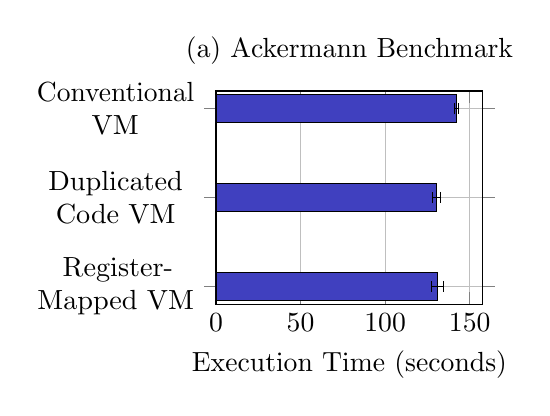
\begin{tikzpicture}
		\begin{axis}[
		title = {(a) Ackermann Benchmark},
		width={0.41\linewidth},
		ytick={1,...,3},
		yticklabels={
			Register-Mapped VM,
			Duplicated Code VM,
			Conventional VM		
			},
		grid=major,
		xbar,
		xlabel=Execution Time (seconds),
		xmin=0,
		y tick label style={text width=2cm,align=center}
		]
		
		\addplot[
		fill=blue!50!gray,
		draw=black,
		every node near coord/.style={inner ysep=5pt},
		error bars/.cd,
		x dir=both,
		x explicit
		] 
		table [x error=error] {
			x   	y	error
			142.25  3	1.20923
			130.431	2	2.17705433
			130.821	1	3.64046
		};
		\end{axis}
		\end{tikzpicture}
		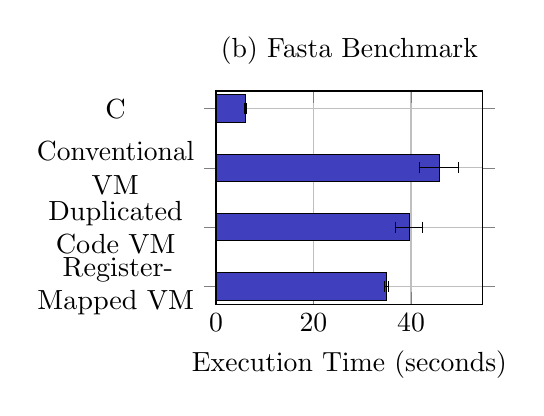
\begin{tikzpicture}
		\begin{axis}[
		title = {(b) Fasta Benchmark},
		width={0.41\linewidth},
		ytick={1,...,4},
		yticklabels={%
			Register-Mapped VM,
			Duplicated Code VM,
			Conventional VM,
			C
			},
		grid=major,
		xbar,
		xlabel=Execution Time (seconds),
		xmin=0,
		y tick label style={text width=2cm,align=center}
		]
		
		\addplot[
		fill=blue!50!gray,
		draw=black,
		every node near coord/.style={inner ysep=5pt},
		error bars/.cd,
		x dir=both,
		x explicit
		] 
		table [x error=error] {
			x   	y	error
			6.113 	4  	0.1539
			45.785  3  	3.974385
			39.63   2	2.7534
			34.956	1	0.35116
		};
		\end{axis}
		\end{tikzpicture}
		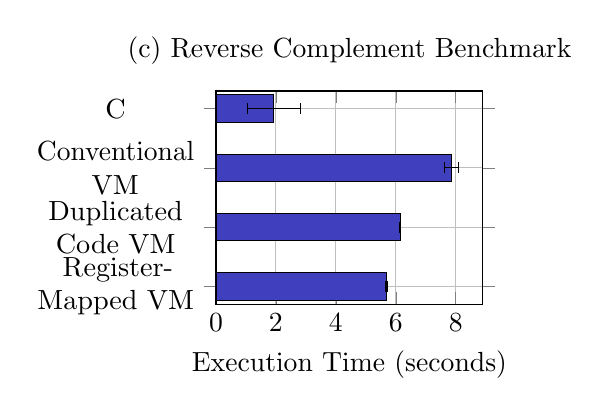
\begin{tikzpicture}
		\begin{axis}[
		title = {(c) Reverse Complement Benchmark},
		width={0.41\linewidth},
		ytick={1,...,4},
		yticklabels={%
			Register-Mapped VM,
			Duplicated Code VM,
			Conventional VM,
			C
		},
		grid=major,
		xbar,
		xlabel=Execution Time (seconds),
		xmin=0,
		y tick label style={text width=2cm,align=center}
		]
		
		\addplot[
		fill=blue!50!gray,
		draw=black,
		every node near coord/.style={inner ysep=5pt},
		error bars/.cd,
		x dir=both,
		x explicit
		] 
		table [x error=error] {
			x   	y	error
			1.925 	4  	0.88735
			7.863  	3  	0.2343
			6.149   2	0.00875
			5.698	1	0.023475
		};
		\end{axis}
		\end{tikzpicture}
		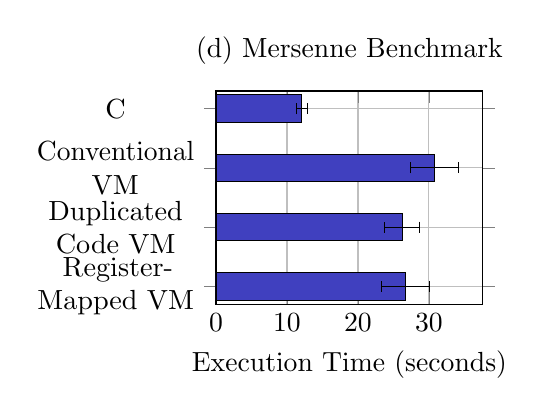
\begin{tikzpicture}
		\begin{axis}[
		title = {(d) Mersenne Benchmark},
		width={0.41\linewidth},
		ytick={1,...,4},
		yticklabels={%
			Register-Mapped VM,
			Duplicated Code VM,
			Conventional VM,
			C
		},
		grid=major,
		xbar,
		xlabel=Execution Time (seconds),
		xmin=0,
		y tick label style={text width=2cm,align=center}
		]
		
		\addplot[
		fill=blue!50!gray,
		draw=black,
		every node near coord/.style={inner ysep=5pt},
		error bars/.cd,
		x dir=both,
		x explicit
		] 
		table [x error=error] {
			x   	y	error
			12.087 	4  	0.79
			30.81	3  	3.36936
			26.229	2	2.47198
			26.718	1	3.394485
		};
		\end{axis}
		\end{tikzpicture}
		
		
		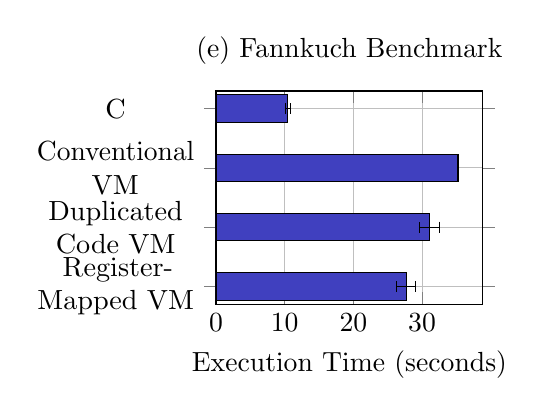
\begin{tikzpicture}
		\begin{axis}[
		title = {(e) Fannkuch Benchmark},
		width={0.41\linewidth},
		ytick={1,...,4},
		yticklabels={%
			Register-Mapped VM,
			Duplicated Code VM,
			Conventional VM,
			C
		},
		grid=major,
		xbar,
		xlabel=Execution Time (seconds),
		xmin=0,
		y tick label style={text width=2cm,align=center}
		]
		
		\addplot[
		fill=blue!50!gray,
		draw=black,
		every node near coord/.style={inner ysep=5pt},
		error bars/.cd,
		x dir=both,
		x explicit
		] 
		table [x error=error] {
			x   	y	error
			10.475 	4  	0.3511
			35.24	3  	0.0828
			31.041	2	1.47051
			27.693	1	1.3622
		};
		\end{axis}
		\end{tikzpicture}
		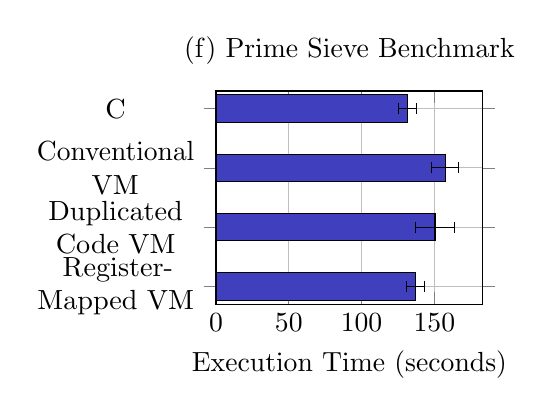
\begin{tikzpicture}
		\begin{axis}[
		title = {(f) Prime Sieve Benchmark},
		width={0.41\linewidth},
		ytick={1,...,4},
		yticklabels={%
			Register-Mapped VM,
			Duplicated Code VM,
			Conventional VM,
			C
		},
		grid=major,
		xbar,
		xlabel=Execution Time (seconds),
		xmin=0,
		y tick label style={text width=2cm,align=center}
		]
		
		\addplot[
		fill=blue!50!gray,
		draw=black,
		every node near coord/.style={inner ysep=5pt},
		error bars/.cd,
		x dir=both,
		x explicit
		] 
		table [x error=error] {
			x   	y   error
			131.628	4  	6.0634
			157.396	3  	9.2844
			150.447	2	13.1281
			137.208	1	6.0634
		};
		\end{axis}
		\end{tikzpicture}
		
		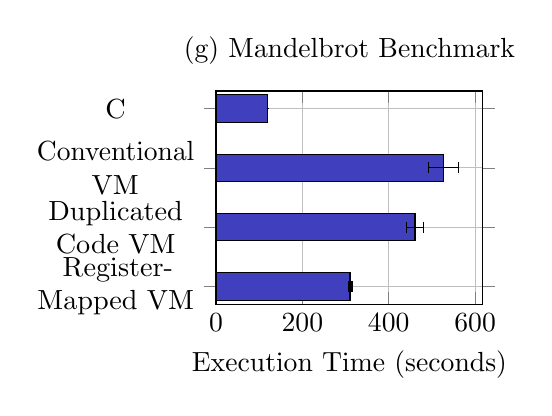
\begin{tikzpicture}
		\begin{axis}[
		title = {(g) Mandelbrot Benchmark},
		width={0.41\linewidth},
		ytick={1,...,4},
		yticklabels={%
			Register-Mapped VM,
			Duplicated Code VM,
			Conventional VM,
			C
		},
		grid=major,
		xbar,
		xlabel=Execution Time (seconds),
		xmin=0,
		y tick label style={text width=2cm,align=center}
		]
		
		\addplot[
		fill=blue!50!gray,
		draw=black,
		every node near coord/.style={inner ysep=5pt},
		error bars/.cd,
		x dir=both,
		x explicit
		]  
		table [x error=error] {
			x   	y   error
			119.761	4  	0.3601
			527.373	3  	34.407
			460.722	2	19.204
			310.399	1	4.4663
		};
		\end{axis}
		\end{tikzpicture}
		\thisfloatpagestyle{empty}
		\caption{Execution Times for Each Benchmark}
		\label{fig:execgraphs}
		\end{myfigure}
	
		Both the duplicated code VM and the register-mapped VM were faster than the conventional VM with all benchmarks. Interestingly, the duplicated code VM and the register-mapped VM offered very little improvement over the conventional VM on the Ackermann benchmark. This may be due to the fact that the Ackermann benchmark performs many \texttt{call} and \texttt{ret} instructions. These instructions have the heftiest implementations, and so the dispatch mechanism takes up a smaller fraction of the total execution time. 
		
		In all the benchmarks except Ackermann and Mersenne, the register-mapped virtual machine was faster than the duplicated code VM. A possible reason for the register-mapped VM being no faster than the duplicated code VM in the Ackermann benchmark is that during a function call and return, the register mapping is broken for the new stack frame. That is, during a function call, the registers are stored in the stack frame (in memory), and the callee takes over control of these registers. Likewise, during function return, registers $g_1$ through $g_4$ are cleared and replaced with the previous values saved in the stack frame. We were unable to think of a more elegant way to implement the \texttt{call} and \texttt{ret} instructions for the register-mapped VM that would make use of the register mapping, and so they are quite slow. This might be an unavoidable disadvantage of the register-mapped design., as registers are in short supply.
		
		It is interesting to compare the difference between execution times on the duplicated code VM and the register-mapped VM. In some benchmarks, such as prime sieve, there is very little difference. This could be because the traversal through the linked list results in a large number of memory loads (to access the `next' pointer in each node), and seldom uses a register for more than very short-term storage (less than ten instructions before a register value is replaced with a value from memory). Register mapping does not contribute much performance gain in this case.
		
		Another interesting comparison to make is the difference in execution time of the C programs from the corresponding benchmark in each VM. This indicates how well suited to each task the virtual machines are. For instance, on the prime sieve benchmark, the virtual machines perform nearly as well as the C program. This suggests that the virtual machine design excels in operations involving pointer operations on the heap.
		
		\reffig{normaltimes} shows the average execution time for each virtual machine. To generate this graph, each benchmark time on each virtual machine was normalised by dividing it by the execution time of the C benchmark. This was done to prevent averages from being unfairly biased towards long-running benchmarks. The graph shows the average of this metric per virtual machine. The Ackermann benchmark is excluded from this graph because the C benchmark never finished. 
		
		\begin{myfigure}
			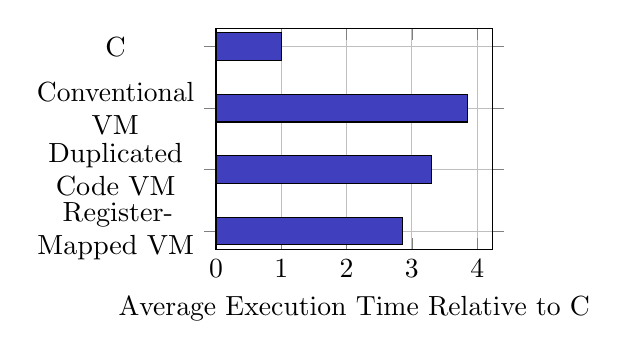
\begin{tikzpicture}
			\begin{axis}[
			width={0.42\linewidth},
			ytick={1,...,4},
			yticklabels={%
				Register-Mapped VM,
				Duplicated Code VM,
				Conventional VM,
				C
			},
			grid=major,
			xbar,
			xlabel=Average Execution Time Relative to C,
			xmin=0,
			y tick label style={text width=2cm,align=center}
			]
			
			\addplot[
			fill=blue!50!gray,
			draw=black,
			every node near coord/.style={inner ysep=5pt},
			]  
			table{
				x   	y
				1	4
				3.847835	3
				3.3		2
				2.86111	1
			};
			\end{axis}
			\end{tikzpicture}
			\caption{Normalised Average Execution Times for Each Benchmark}
			\label{fig:normaltimes}
		\end{myfigure}
		
		The graph shows that both the register-mapped VM and the duplicated code VM performed better than the conventional VM compared to native execution on average. The register-mapped VM performed better than the duplicated code VM on average. All virtual machines were more than twice as slow as the native C programs, on average.
	
		\subsection{Cache Behaviour}
		The Cachegrind results were very encouraging. None of the programs showed any significant instruction cache misses---under 0.01\% of all instruction loads resulted in a cache miss. There was an expectation to see more instruction cache misses because of the large code size, but there is a possible explanation for its absence. Though there is a large amount of implementation code, a typical assembly program will not dynamically use all instruction-operand combinations. It is not necessary for the processor to cache the implementation code that is not used by the program, so a large percentage of the code does not even make it into the cache. This frees up space for code that does need to be cached.
		
		\subsection{Branch Target Prediction}
		Cachegrind is also able to simulate the branch prediction behaviour of programs. Cachegrind was used to characterise the indirect branch prediction behaviour. The frequency of indirect branches that were predicted correctly, and those that weren't, are graphed in \reffig{btbgraph}. The indirect branch behaviour of the native C programs is not reported here, because it doesn't contribute to the discussion of the predictability of virtual machines.
		
		\begin{myfigure}
			\pgfplotsset{scaled x ticks=false}
			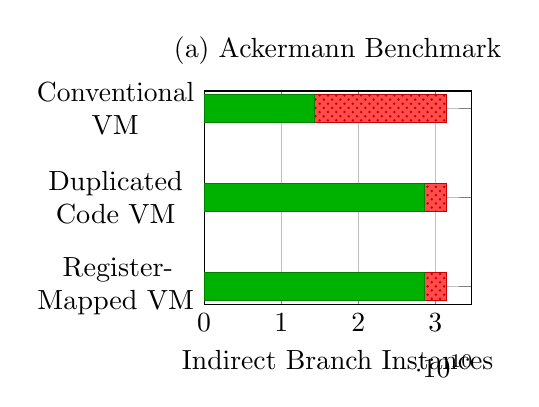
\begin{tikzpicture}
			\begin{axis}[
			title = {(a) Ackermann Benchmark},
			width={0.41\linewidth},
			ytick={1,...,3},
			yticklabels={
				Register-Mapped VM,
				Duplicated Code VM,
				Conventional VM
			},
			grid=major,
			xbar stacked,
			xlabel=Indirect Branch Instances,
			xmin=0,
			y tick label style={text width=2cm,align=center}
			]
			
			\addplot[
			fill=green!70!black,
			draw=green!50!black,
			every node near coord/.style={inner ysep=5pt},
			] 
			table {
				x	y
				28629447240		1
				14314985800		3
				28629447240		2
			};
			\addplot[
			fill=red!70,
			draw=red!80!black,
			postaction={
				pattern=crosshatch dots,
				pattern color=red!80!black
			},
			every node near coord/.style={inner ysep=5pt},
			] 
			table {
				x	y
				2863442739	1
				17177904179	3
				2863442739	2
				
			};
			
			\end{axis}
			\end{tikzpicture}
			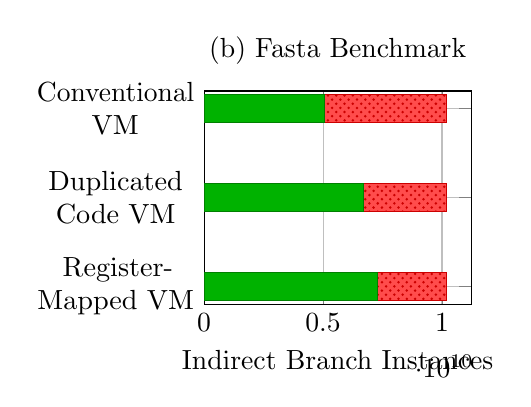
\begin{tikzpicture}
			\begin{axis}[
			title = {(b) Fasta Benchmark},
			width={0.41\linewidth},
			ytick={1,...,4},
			yticklabels={%
				Register-Mapped VM,
				Duplicated Code VM,
				Conventional VM
			},
			grid=major,
			xbar stacked,
			xlabel=Indirect Branch Instances,
			xmin=0,
			y tick label style={text width=2cm,align=center}
			]
			
			\addplot[
			fill=green!70!black,
			draw=green!50!black,
			every node near coord/.style={inner ysep=5pt},
			]
			table{
				x	y
				7279455249		1
				5045052543		3
				6682704349		2				
			};
			\addplot[
			fill=red!70,
			draw=red!80!black,
			postaction={
				pattern=crosshatch dots,
				pattern color=red!80!black
			},
			every node near coord/.style={inner ysep=5pt},
			] 
			table {
				x	y
				2923312485	1
				5157715191	3
				3520063385	2
			};
			\end{axis}
			\end{tikzpicture}
			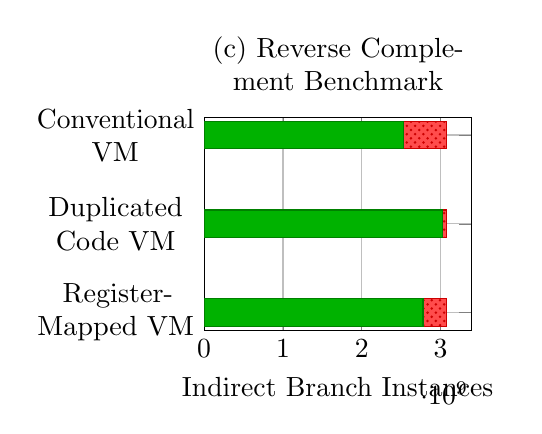
\begin{tikzpicture}
			\begin{axis}[
			title = {(c) Reverse Complement Benchmark},
			width={0.41\linewidth},
			ytick={1,...,4},
			yticklabels={%
				Register-Mapped VM,
				Duplicated Code VM,
				Conventional VM
			},
			grid=major,
			xbar stacked,
			xlabel=Indirect Branch Instances,
			xmin=0,
			y tick label style={text width=2cm,align=center},
			title style={text width=0.35\linewidth,align=center}
			]
			
			\addplot[
			fill=green!70!black,
			draw=green!50!black,
			every node near coord/.style={inner ysep=5pt},
			] 
			table{
				x	y
				2777331430		1
				2527207846		3
				3025248687		2
				
				
			};
			\addplot[
			fill=red!70,
			draw=red!80!black,
			postaction={
				pattern=crosshatch dots,
				pattern color=red!80!black
			},
			every node near coord/.style={inner ysep=5pt},
			] 
			table {
				x	y
				302084202	1
				552207786	3
				54166945	2
				
			};
			\end{axis}
			\end{tikzpicture}
			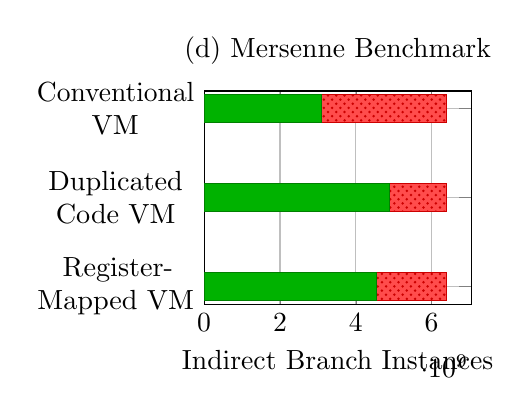
\begin{tikzpicture}
			\begin{axis}[
			title = {(d) Mersenne Benchmark},
			width={0.41\linewidth},
			ytick={1,...,4},
			yticklabels={%
				Register-Mapped VM,
				Duplicated Code VM,
				Conventional VM
			},
			grid=major,
			xbar stacked,
			xlabel=Indirect Branch Instances,
			xmin=0,
			y tick label style={text width=2cm,align=center}
			]
			
			\addplot[
			fill=green!70!black,
			draw=green!50!black,
			every node near coord/.style={inner ysep=5pt},
			] 
			table {
				x	y
				4549678295		1
				3100143151		3
				4899360247		2
			};
			\addplot[
			fill=red!70,
			draw=red!80!black,
			postaction={
				pattern=crosshatch dots,
				pattern color=red!80!black
			},
			every node near coord/.style={inner ysep=5pt},
			] 
			table {
				x	y
				1851826825	1
				3301361969	3
				1502144873	2
			};
			\end{axis}
			\end{tikzpicture}
			
			
			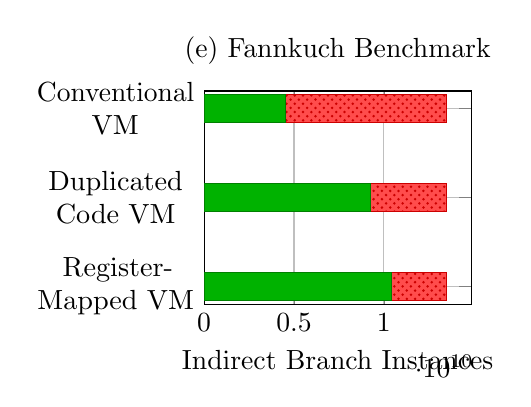
\begin{tikzpicture}
			\begin{axis}[
			title = {(e) Fannkuch Benchmark},
			width={0.41\linewidth},
			ytick={1,...,4},
			yticklabels={%
				Register-Mapped VM,
				Duplicated Code VM,
				Conventional VM
			},
			grid=major,
			xbar stacked,
			xlabel=Indirect Branch Instances,
			xmin=0,
			y tick label style={text width=2cm,align=center}
			]
			
			\addplot[
			fill=green!70!black,
			draw=green!50!black,
			every node near coord/.style={inner ysep=5pt},
			] 
			table {
				x	y
				10437208229		1
				4517212205		3
				9244315131		2
			};
			\addplot[
			fill=red!70,
			draw=red!80!black,
			postaction={
				pattern=crosshatch dots,
				pattern color=red!80!black
			},
			every node near coord/.style={inner ysep=5pt},
			] 
			table {
				x	y
				3069689230	1
				8989685254	3
				4262582328	2
			};
			\end{axis}
			\end{tikzpicture}
			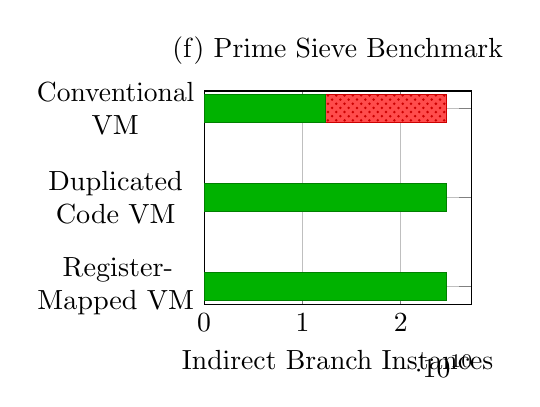
\begin{tikzpicture}
			\begin{axis}[
			title = {(f) Prime Sieve Benchmark},
			width={0.41\linewidth},
			ytick={1,...,4},
			yticklabels={%
				Register-Mapped VM,
				Duplicated Code VM,
				Conventional VM
			},
			grid=major,
			xbar stacked,
			xlabel=Indirect Branch Instances,
			xmin=0,
			y tick label style={text width=2cm,align=center}
			]
			
			\addplot[
			fill=green!70!black,
			draw=green!50!black,
			every node near coord/.style={inner ysep=5pt},
			] 
			table {
				x	y
				24686942677		1
				12346481823		3
				24687099667		2
			};
			\addplot[
			fill=red!70,
			draw=red!80!black,
			postaction={
				pattern=crosshatch dots,
				pattern color=red!80!black
			},
			every node near coord/.style={inner ysep=5pt},
			] 
			table {
				x	y
				3314133	1
				12343774987	3
				3157143	2
			};
			\end{axis}
			\end{tikzpicture}
			
			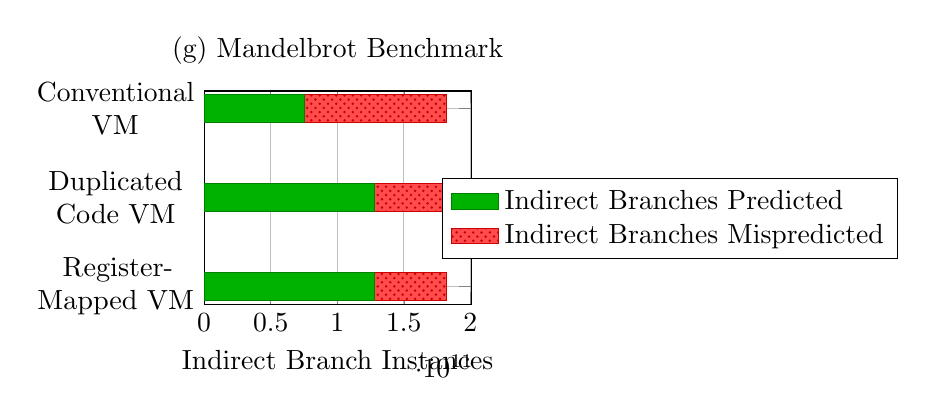
\begin{tikzpicture}
			\begin{axis}[
			title = {(g) Mandelbrot Benchmark},
			width={0.41\linewidth},
			ytick={1,...,4},
			yticklabels={%
				Register-Mapped VM,
				Duplicated Code VM,
				Conventional VM
			},
			grid=major,
			xbar stacked,
			area legend,
			legend style={
				at={(2.6,0.4)},
				anchor=east,
				legend cell align=left
			},
			xlabel=Indirect Branch Instances,
			xmin=0,
			y tick label style={text width=2cm,align=center}
			]
			
			\addplot[
			fill=green!70!black,
			draw=green!50!black,
			every node near coord/.style={inner ysep=5pt},
			]
			table {
				x	y
				128183200940		1
				75257786444		3
				128183216939		2
			};
			\addlegendentry{Indirect Branches Predicted}
			\addplot[
			fill=red!70,
			draw=red!80!black,
			postaction={
				pattern=crosshatch dots,
				pattern color=red!80!black
			},
			every node near coord/.style={inner ysep=5pt},
			] 
			table {
				x	y
				54104775594	1
				107030190090	3
				54104759595	2
			};
			\addlegendentry{Indirect Branches Mispredicted}
			\end{axis}
			\end{tikzpicture}
			\thisfloatpagestyle{empty}
			\caption{Indirect Branch Prediction for Each Benchmark}
			\label{fig:btbgraph}
		\end{myfigure}
		
		The virtual machines all performed a similar number of indirect branches for each benchmark. However, 50\% of the conventional VM's indirect branches were mispredicted on average, whereas the register-mapped VM and the duplicated code VM's indirect branches were mispredicted 18.4\% and 18.6\% respectively. This is a dramatic difference. The processor was far more successful in predicting the behaviour of the duplicated code and the register-mapped machine than it was with the conventional VM.
		
		In the prime sieve benchmark, the graphs may mislead one into thinking that the duplicated code VM and the register-mapped VM did not mispredict any indirect branches. In fact, they mispredicted a tiny fraction of indirect branches: around 0.01\% in both cases.
		
		The branch prediction performance gain experienced by the duplicated code and register-mapped VM compared to the conventional VM varies with benchmark. It is possible that this could be attributed to differing levels of predictability in the loops of each benchmark. For instance, some benchmarks may contain loops with the exact same instruction twice. This problem was discussed earlier, and such a situation does exist in some of the benchmarks programs.
		
% Last chapter
\chapter{Conclusion}
	All virtual machines were around three times as slow as the C programs, on average. This is actually a surprisingly good result, since virtual machines tend to be around five to ten times slower than a native program. It is possible that implementing the virtual machines in assembly caused all the virtual machines to be very efficient, because assembly programs tend to be very lightweight compared to those written in a high-level language.
	
	The results show that conventional register virtual machines can be improved by modifying their design to leverage new design features of modern processors---for instance---large amounts of instruction cache. Duplicating implementation code was very effective at reducing the proportion of mispredicted indirect branches, without having a meaningful impact on the ability of the processor to cache the virtual machine's implementation code. The virtual machines with duplicated code were, on average, 60\% more predictable than the conventional virtual machine.
	
	The reason duplication had such a significant impact is supported by theory. Increasing the number of implementations increases the likelihood that a particular dispatch instance will branch to a unique implementation, simply because the virtual machine consists of implementations which are more specific---it is not often that the exact same instruction/operand combination occurs in many places in the program bytecode. This results in overall increased indirect branch prediction accuracy. 
	
	We are able to do this without sacrificing instruction cache performance, because of the large amount of instruction cache available on modern processors. In fact, no virtual machine had a problem becoming almost entirely cached (at least, the parts that were actually used), which is in stark contrast to the worries of past researchers. This in indicative of the large shift in processor design over the last twenty years.
	
	A second source of performance improvement is achieved by the elimination of the instruction decode step, and---in the register-mapped VM---operand fetch and store. In addition to the execution time saved by skipping these steps, their elimination also reduces the amount of data dependence on the behaviour of the virtual machine, making it easier for the processor to perform speculative optimisation. For instance, the processor can load the value of operands before they are needed by the instruction's implementation. If a virtual machine needs to decode instructions, the processor is only able to load these values after the bytecode instruction has been decoded and the involved operands determined.
	
	Register mapping also improves the performance of virtual machines, although not to the extent we expected. \todo{add average data here} Keeping the often-accessed virtual machine registers in high-speed hardware registers caused this improvement. We have a possible explanation for the small margin between the register-mapped and duplicated code VM. In the duplicated code VM, the virtual registers in main memory are almost certainly going to be cached in L1 data cache. This reduces the performance penalty of storing virtual registers in main memory significantly, and closes the performance gap between the duplicated code and register-mapped VM. However, the register-mapped VM is still a solid improvement over the duplicated code VM, which constitutes a positive result.
	
	\section{Opportunities for Future Development}
	These results demonstrate that there are still useful techniques to be discovered in the field of non-JIT interpreters. It is important to mention that ``non-JIT techniques'' are not irrelevant in a landscape dominated by JIT interpreters. Rather, these techniques complement JIT techniques, and should be pursued in the interests of producing performant interpreters on modern architectures.
	
	Assembly programming has lost favour amongst developers because of its difficulty and declining benefit caused by the improved optimisation ability of modern compilers. It is thus likely that interpreter developers may be unwilling to implement their virtual machines in assembly. However, some of the ideas investigated in this research---especially the code duplication aspect---are still applicable in high-level languages like C. For this reason, it would be beneficial to investigate the introduction of these ideas into existing virtual machines.
	
	It was surprising to discover instruction cache misses did not affect performance of the VM. Considerable design effort and compromise was exercised to reduce the number of instructions in the VM architecture. It would be interesting to see how big a virtual machine implementation can get before instruction cache becomes an important issue. This will help to see whether large virtual machines can be used in a practical VM architecture with many more pragmatic instructions.
	
	\clearpage
	\section{Reflection}
	If one thing was determined by this study, it is that the old wisdom of interpreter design needs to be revisited in light of the emergence of modern processor design. Ideas that were thought infeasible twenty years ago may be surprisingly effective today. For instance, the core idea which resulted in the encouraging results that were achieved were dismissed by \cite{stackcaching}. The points made by Ertl were valid in 1995, but technology has changed substantially since then.
	
	However, the advent of ever-increasing complexity of modern processors comes at a cost---discovering the exact mechanism by which modern processors achieve their performance is proprietary knowledge of their manufacturers. Producing designs which fully leverage these ``secret optimisation features'' is a frustrating task, because so little is known about their implementation.
	
	
	
% Bibliography
\bibliographysection

\end{document}